\chapter{Introduction}
\renewcommand{\baselinestretch}{\mystretch}
\label{chap:Intro}
%\setlength{\parindent}{0pt}

\PARstart{F}{uzz} testing, also known fuzzing test, is a kind of software test technique that involves providing invalid, unexpected or random data as input to a compiler \cite{miller2007fuzz}. As a quality assurance technique, fuzz testing is efficient to find the coding errors and security loopholes in the compiler even in high level operating systems and networks. With large amount of random input data, the under tested device is attempt to crash or suffering memory overflow issue. If a vulnerability is detected in the software, the potential cause of the crash or error is also need to be identified. The identification is to located the error and comparing the influence with the error reference table. The ''fuzzer'' is defined to generate the large random inputs and identify the potential cause of the error or crash. Due to the acknowledge of the device under test (DUT)'s inside structure, the fuzzer can be categorised as white-box, grey-box and black box.

In conventional hardware design, the truth table and boolean expression need to be simplified manually and realised in real logical gate circuit. This process is cumbersome and error-prone. By working in a high abstract level which means only specific the logic function and involved the computer aided design (CAD) can greatly improve the design efficiency and reduce the number of design errors \cite{harris2015digital}. 
The modern hardware design and verification is heavily reliant on the HDL such as Verilog, SystemVerilog and VHSIC (Very High Speed Integrated Circuit) Hardware Description Language (VHDL). As a mainstream HDL, Verilog was standardised as IEEE 1364 in 2009 \cite{1620780} which occupied a large market share in industry and commercial application area. In 2009 the Verilog standard (IEEE 1364-2005) was merged with SystemVerilog standard and officially become a part of SystemVerilog. Since, a new standard was formed as IEEE 1364-2005. Comparing with VHDL, Verilog has more compact statements and more flexibility. As a consequence, the Verilog was chosen as the HDL in this project. The HDL code file needs to be transformed to a netlist by a hardware synthesis tool, for example VIVADO and ModelSim. The correctness of synthesis is the basis of the electronic production. It is important to design a test algorithm for the hardware synthesis tool.
% JW: But *why* is it important? It's crucial that you explain this to your readers. Why do hardware synthesisers need testing? What might happen if they have bugs?
\section{Motivation}
% JW: Aha, this is what I was missing earlier! Ok, the following subsection needs to come *much* earlier. The first thing you need to do in your report is convince your readers that you are solving an important problem. Once you have done this, *then* you can talk about your solution (which is fuzzing).
First of all, the high reliability of the synthesis tool is important to the synthesised circuit. Hoang M. et al have shown that most of the incorrect generations of netlist related to the Trojans in synthesis tool rather than invalid HDL code \cite{torjans}. Despite the development of self-verification, external testing is necessary. For instance, Intel's famous floating point division (FDIV) bug in the Pentium processor was discovered by Prof. Thomas R. Nicely at Lynchburg College \cite{Intelbug}. Due to this bug, the processor may process a wrong result when dividing a number. The incorrect calculated result occurring probability is 1 in 9 billion FDIV with random parameters. As estimated, recalling the defect processors and replacement them costed Intel company approaching 475 million dollars. Lack of third-party verification and testing may cause the synthesis tool become even more error-prone.

Secondly, the existing testing tool has several limitations. The coverage of the test is narrow. For the existing synthesis tool testing software, VlogHammer's generations are concentrated on combinatorial circuit with small number of ports and terminals. Large scale of fuzz input may more effective than original method. 

In addition, this project has comprehensive research foreground 
% JW: What does "comprehensive research foreground" mean?
and potential value.
% JW: "potential value" is too vague -- be more specific about what the value is.
Big data analytic offers effective statistical power and can be used in predictive analytic and user behaviour analytic. In future, the investigation of performance of the fuzzer and the detected vulnerabilities identification can be matured by big data analytic. This cross subject analysis may shedding light on what feature of the fuzz testing algorithm need to be developed related to bug-hunting ability.
\section{Fuzzing in hardware synthesis}
In 1989, the fuzz testing algorithm was initially proposed by Barton Miller at University of Wisconsin \cite{miller2007fuzz}. He designed a fuzzer to automatically generate random file and command lines to test the utility of an Unix-based application. The debugging tool to identify the cause of crash was also provided by him. As presented in his paper \cite{miller1990empirical}, 25-33\% of the utility programs on different version of UNIX system were crashed during the fuzz testing. Above results shows that this testing algorithm is effective to finding the bugs existed in the DUT. At present, the definition of term fuzz testing is not limited in the command-line utilities.
Although the weakness of the fuzz testing algorithm is the bug-finding pertinence is not robust. 
% JW: What do you mean by "bug-finding pertinence"?
With the simple design structure, high practicability and capability, it has impressive cost-efficient ratio in debugging area to discover severe overlooked defects. Different from other testing algorithm and method, it has advantage that does not need oracle for test results. For software testing, the main application of this testing algorithm is to discover the vulnerabilities such as buffer overflow,
denial of service (DOS), cross-site scripting and structured query language (SQL) injection\cite{Yang:2011:FUB:1993316.1993532}. 

Based on above discussion, the purpose of this project is to apply this fuzz testing algorithm in hardware synthesis tool. With the trend of open source project(OPS), this project is focusing on low-level open-source hardware synthesis software for example, ABC and SIS. The random generated HDL files will be entered to a hardware synthesis software by a bash shell program. Inspired by Xuejun Yang and his colleagues designed Csmith \cite{Yang:2011:FUB:1993316.1993532}, the basic block diagram of this project shows in Fig \ref{Fig:Block diagram}. On the left-hand side, GNC compiler collection (GCC) and Microsoft's Visual studio (MSV) are C compilers and on the right-hand side, ABC and SIS are hardware synthesis software. Different from the software fuzz testing, the input netlist file can directly comparing with the output of the hardware synthesis tool. Because these two files are in same format and easy to do the function test. Comparing the synthesised netlist with its original input circuit, if these two circuits are not equivalent, it indicates that might be a bug existing in the tested tool. 
% JW: The figure is nicely drawn, but it doesn't actually reflect your toolflow. On the left-hand side you're comparing the outputs of *two different* C compilers. But in your toolflow, you only need *one* hardware synthesiser, because you compare the *input* of the tool against its *output*. You're not comparing the output of ABC against the output of SIS, which is what your diagram shows.

\begin{figure}[htb]
\centering
\begin{minipage}[htb]{1\textwidth}
\centering
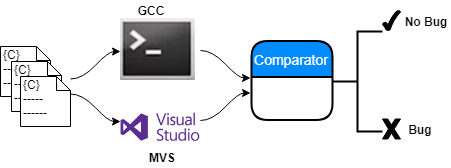
\includegraphics[width=8cm]{MScThesisTemplate/Figs/1.png}
\end{minipage}
\begin{minipage}[htb]{1\textwidth}
\centering
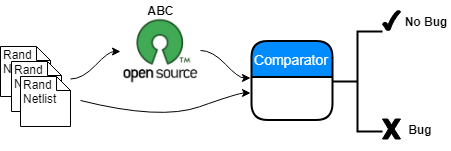
\includegraphics[width=8cm]{MScThesisTemplate/Figs/2.png}
\end{minipage}
\caption{Block diagram}
\label{Fig:Block diagram}
\end{figure}

\section{Project Contribution}
The main contributions of this project are:
\begin{itemize}
    \item Applying the fuzz testing algorithm in open-source hardware synthesis tool testing field. The fuzz testing method's state of art was advanced and extended. The random generated file has better coverage and more esoteric comparing to typical Verilog code file generated by existing testing tool.
    \item Detected bugs and crash issue were analysed through qualitative and quantitative. Not only benefits the debug and version updating for the hardware synthesis tool, but also worthy in big data research in bug-hunting. 
    \item With further polishing, the designed testing tool can be promoted as a distributed Linux software in a collaborative public manner.
\end{itemize}

\section{Thesis Outline}
This thesis is divided into 6 chapters to illustrate the design and implementation of the fuzzing netlist. Following the first introduction, the background chapter 2 will demonstrate the theory applied in this project with the literature review. Chapter 3 discuss the project plan including the objectives and strategy for evaluating the project. In Chapter 4 the detail implementation of combinational and sequential testing circuit with high-level coding language. The bash shell program with error detection will also be presented. The result and future improvement of designed the fuzzer and toolflow will be depicted and evaluated in Chapter 5. In the final chapter 6, it conclude the impact of the project and future work. 